\section{Discussion} \label{sec:Discussion}
\subsection{Caveats}
This work and its results cannot be blindly trusted. There are a few assumptions and problems in the course of the investigations which might have influenced the results.
\\\\\textbf{GC selection:}
One of the main problems in the analysis is the \acp{GC} selection. We applied a very simple recipe which only excluded \acp{GC} which were in a snapshot in a regime where the disk forces were very strong and should have destroyed the \ac{GC}. When selecting only a subset of the \acp{GC}, we have very different statistics of each progenitor group, e.g. the means shift significantly. A proper, physical selection would make these results more reliable. 
\\\\\textbf{Potential fit:}
As we have discussed in Section \ref{subsec:wrong_pot_fit}, there are a few problems with the potential fit. The decomposition probably underestimates but also flares out the disk. For each component, the model differs from the data especially in the center. This is due to the choice of binning the data, fitting routines, etc. In total, the potential is good enough for the course of our investigations but, as one of the next steps, should be improved.
\\\\\textbf{Cold vs hot streams:}
The assumption that the \ac{DF} of the \acp{GC} is a $\delta$-function requires them to be like a cold stream. Already in the introduction we have mentioned, that \ac{DG} mergers usually create hot streams so our \acp{GC} are probably dynamically hot and have a different, more complex \ac{DF}.
\textbf{}
\subsection{Comparison to observations}
It is import to compare results from analysis simulations to observations. One test is looking at our Galaxy, where we have 6D phase space information available, and to see how remnants of a \ac{DG} merger distributed actions space.
\iffalse
\textbf{Excursion: coordinate transformations}
private communication with Wilma Trick
\fi
Recently, \textit{Gaia}-Enceladus \citep{Enceladus....Helmi...2018} \textcolor{red}{also put in references of sausage DG} was discovered in the \textit{Gaia} data. These are remnant stars of a merger approximately \SI{10}{Gyr} ago with a mass ratio of 0.24. 

\begin{figure}[htbp]
    \centering
    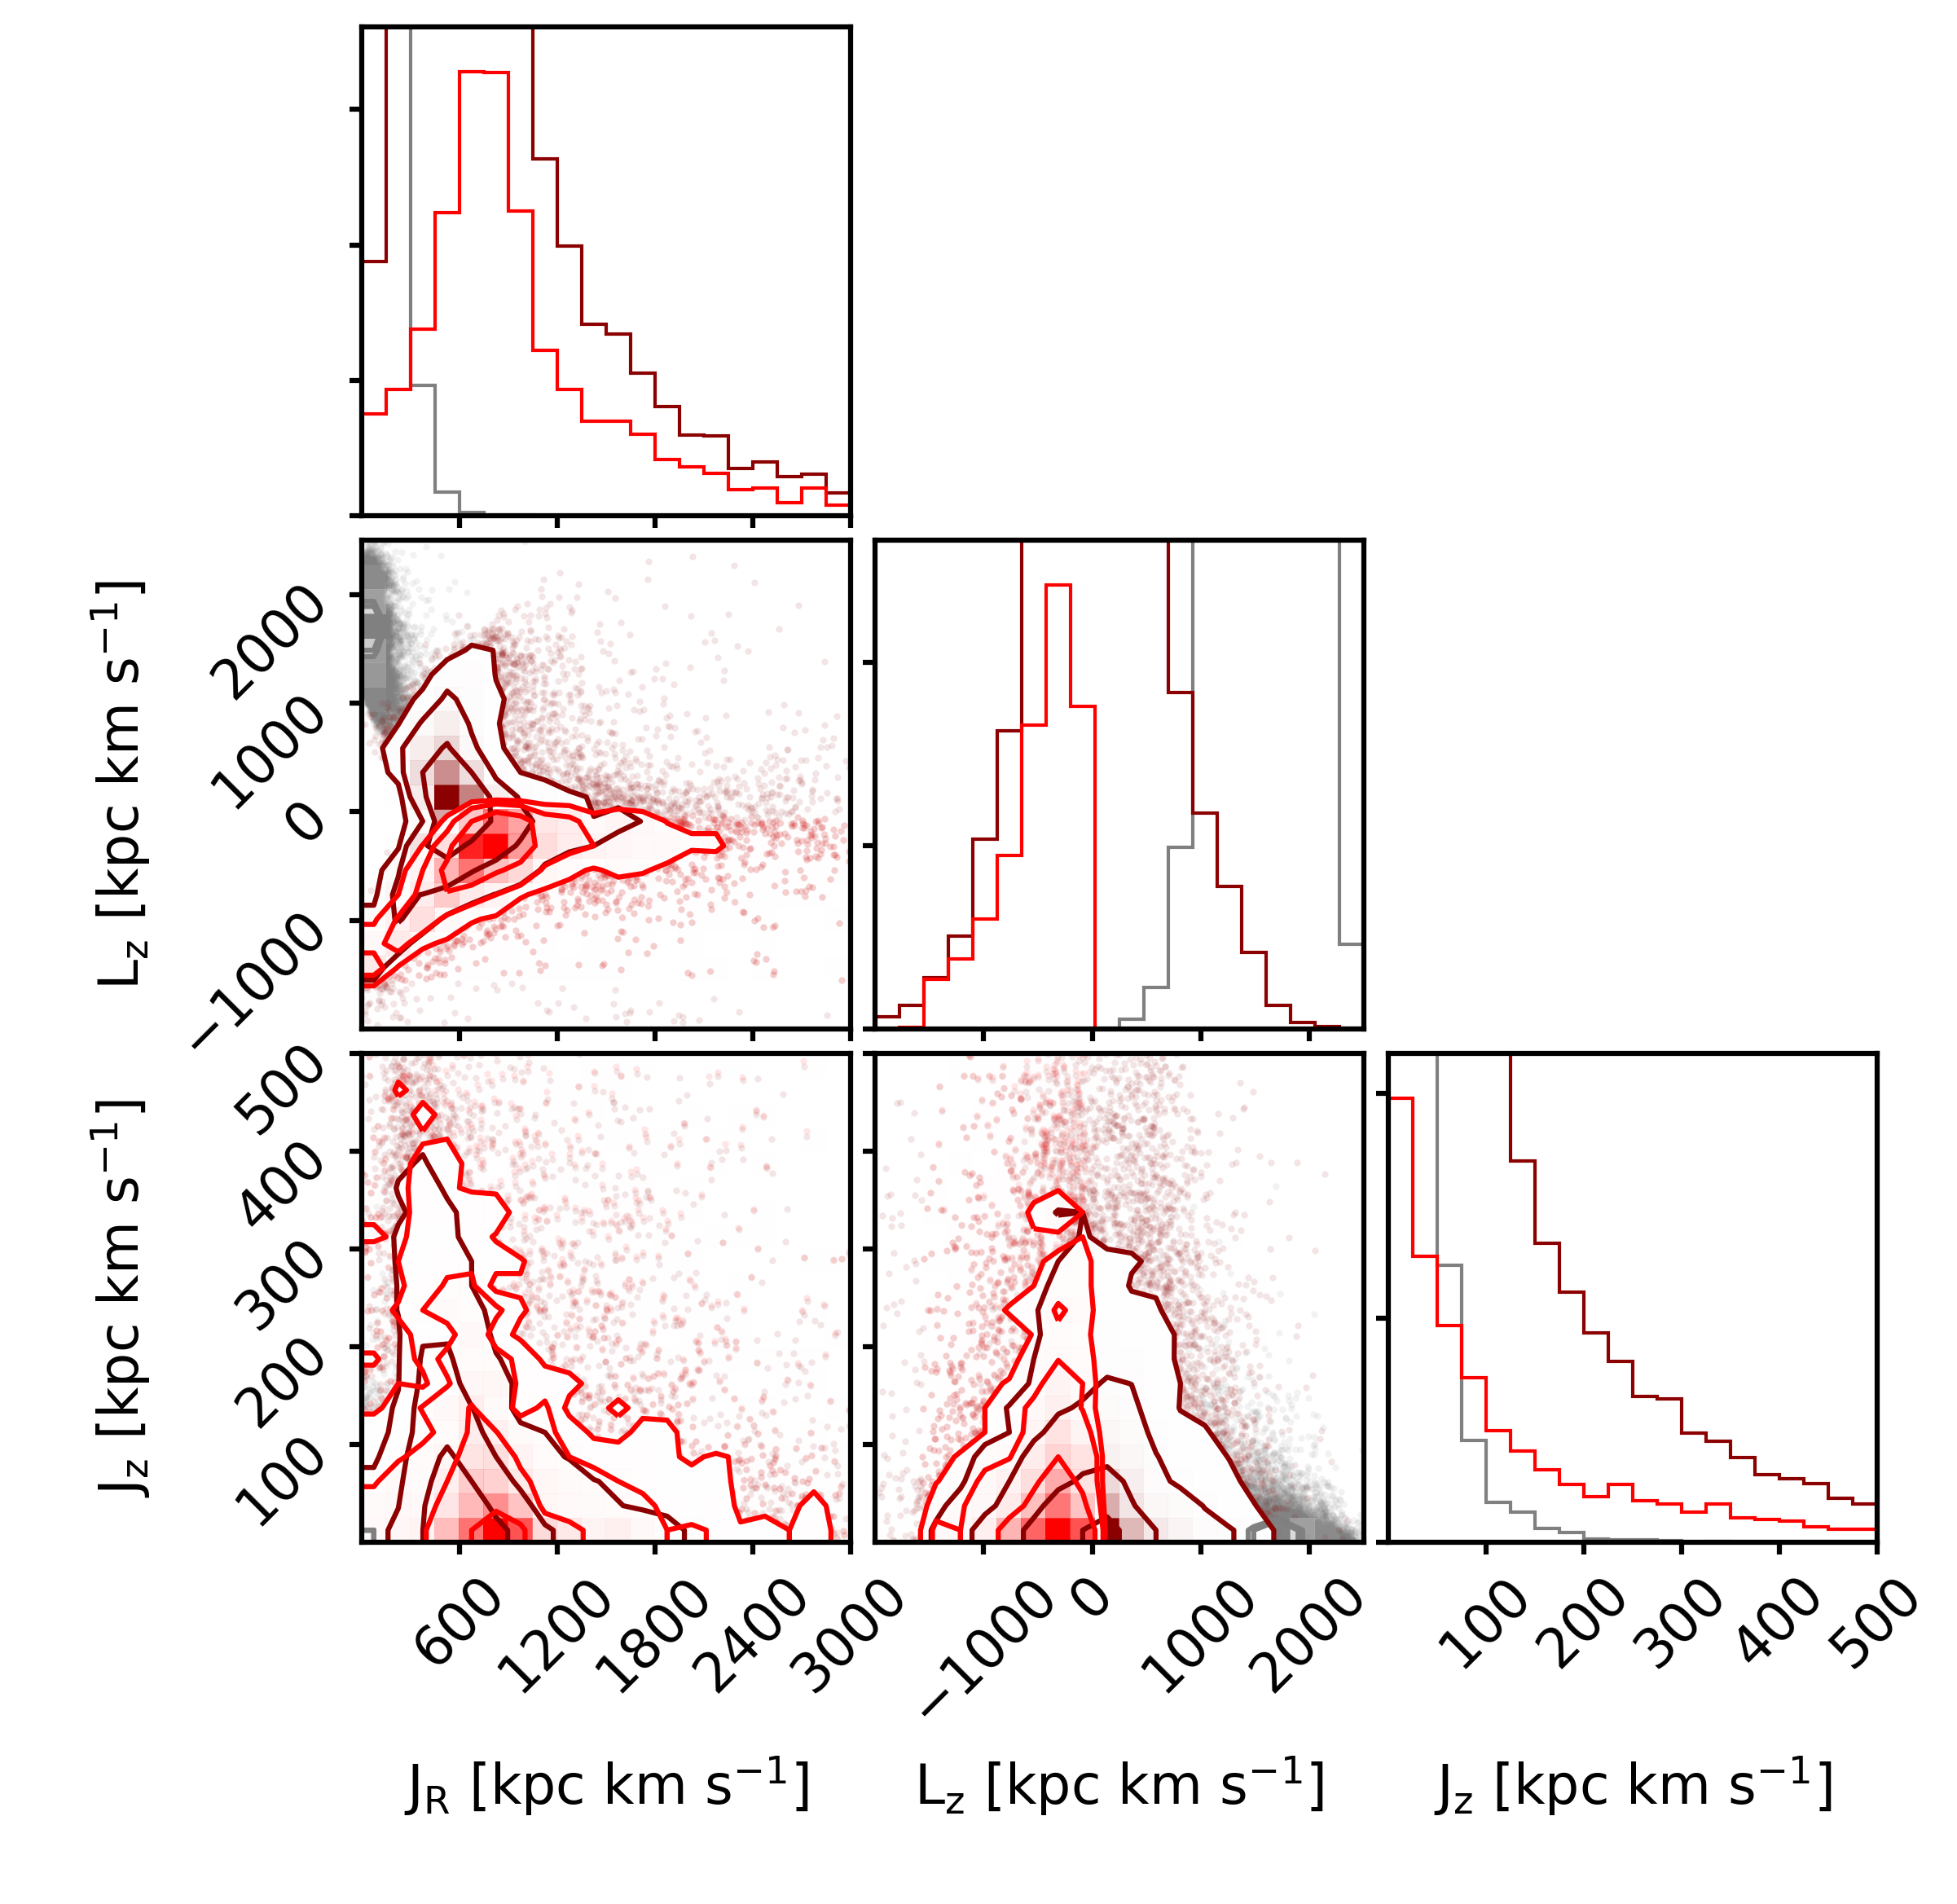
\includegraphics[width=1.0\textwidth]{plots/Discussion/Gaia_all_actions_MW14_talk3.png}
    \caption{\textit{Gaia}-Enceladus stars in action space in the galpy MW14Potential. In grey, actions of disk stars are plotted. Dark red is the halo including some of the thick disk stars. \textit{Gaia}-Enceladus stars are plotted in red. Disk and halo are clearly distinguishable in angular momentum and also in radial action. \textit{Gaia}-Enceladus is not distinguishable from the halo as it makes up a significant part of it. It is also very spread out in action space so we cannot detect any sharp features.}
    \label{fig:Gaia_Enceladus_actions}
\end{figure}
We show in Figure \ref{fig:Gaia_Enceladus_actions} actions of the disk, halo and \textit{Gaia}-Enceladus. The remnants are neither distinguishable from the halo nor do they make a sharp feature in any of the actions. This tells us that even if there was more dynamical information contained in these stars shortly after the merger, this information vanishes over time.


\subsection{Comparison to literature and other work}
\textbf{\acp{GC} formation in cosmological simulations} Timo Halbesma (PhD student at the MPA) is working on extracting \acp{GC} in the Auriga simulations which have proper physical properties and reasons to exist. Doing the same analysis with a set of proper \acp{GC} could change our results drastically. One reason could be that our population samples are too big and another one could be that if we select properly surviving \acp{GC} they could clump in action space because their orbits might stay constant and be properly affected by potential changes.\\
The E-MOSAICS simulation suite \citep{Pfeffer...E-MOSAICS...2018, Kruijssen...E-MOSAICS.MW..2018} are zoom-in simulations of the cosmological EAGLE \citep{Schaye...EAGLE...2015} simulations which have implemented models describing the formation, evolution, and disruption of star clusters. In these simulations, Meghan Hughes (PhD student at ESO/LJMU) works on modelling the potential and Sebastian Trujillo-Gomez (Post-doc at ARI) investigates the action of the \acp{GC}. 
\\\\
\textbf{Constraining gravitational potential}
\textcolor{red}{sorry muss hier noch in die literatur schauen}
There are attempts of applying adaptive dynamics to the \ac{MW}.
\begin{itemize}
    \item \textbf{\acp{DF} of \acp{GC}} \citep{Posti...MWmassGCs...2018}
    looked at all GCs and did not differentiate bw in-situ/ex-situ and coming from differetn \acp{DG}
    \item \textbf{Sharpen stellar streams in sims to find true potential} \citep{Sanderson...streams..adaptivedyn...2015, Sanderson...gravpotstreams...2017}
\end{itemize}


\subsection{Future Work}
There are a lot of things which we could not investigate or we had to make compromises on due to the time limitations of this thesis. Big issues which we already discussed are with the potential model and with the \ac{GC} selection. Improving these recipes would make our analysis more robust.
\\\\
galpy and AGAMA \citep{Vasiliev...AGAMA...2019} can calculate actions for \textit{N}-body simulations directly without the need of an analytic gravitational potential. We should compare if the action distribution and evolution behaves as we measured because of their nature and their physical evolution in the simulation (so direct calculation of actions and calculating them in the potential model would give similar results) or because a analytic axisymmetric potential (in general or only our fit) comes not close to reality and messes these things up. Up to now, it was not possible to do this step because of technical issues. 

\\\\The final goal would be to find the right \ac{DF} of accreted particles which is not yet possible due to numerical (and observational) limitations. If we had that, adaptive dynamics in external galaxies should be a useful method to constrain their gravitational potential. With this true \ac{DF} and the right gravitational potential, we would know everything about the dynamics of the galaxy.

